%-------------------------------------------------------
%    DOCUMENT CONFIGURATIONS
%-------------------------------------------------------

%-------------------------------------------------------
%    START OF COMMUNICATION
%-------------------------------------------------------
\subsection{Communication}

During the analyze, it was concluded that the best solution would be to have a consensus-driven list of nodes. We focused during this project on the base of the communication between node. We then started with the PeerJS' Open Source technology that allows us to run in the cloud or on personal servers a signaling server with simple APIs. During the prototyping and testing, we had the pleasure to find a serverless procedure for signaling.

\subsubsection{PeerJS} The first version of the prototype used PeerJS' APIs and its free server for developers (maximum of 50 concurrent connections). Note that developers are encouraged to run their own signaling servers. The figure ~\ref{img:basic-signaling} schematize what was implemented.
\begin{figure}[htpb]
\centering
\caption{\small \sl Basic Signaling Scheme
\label{img:basic-signaling}}
\begin{adjustbox}{center}
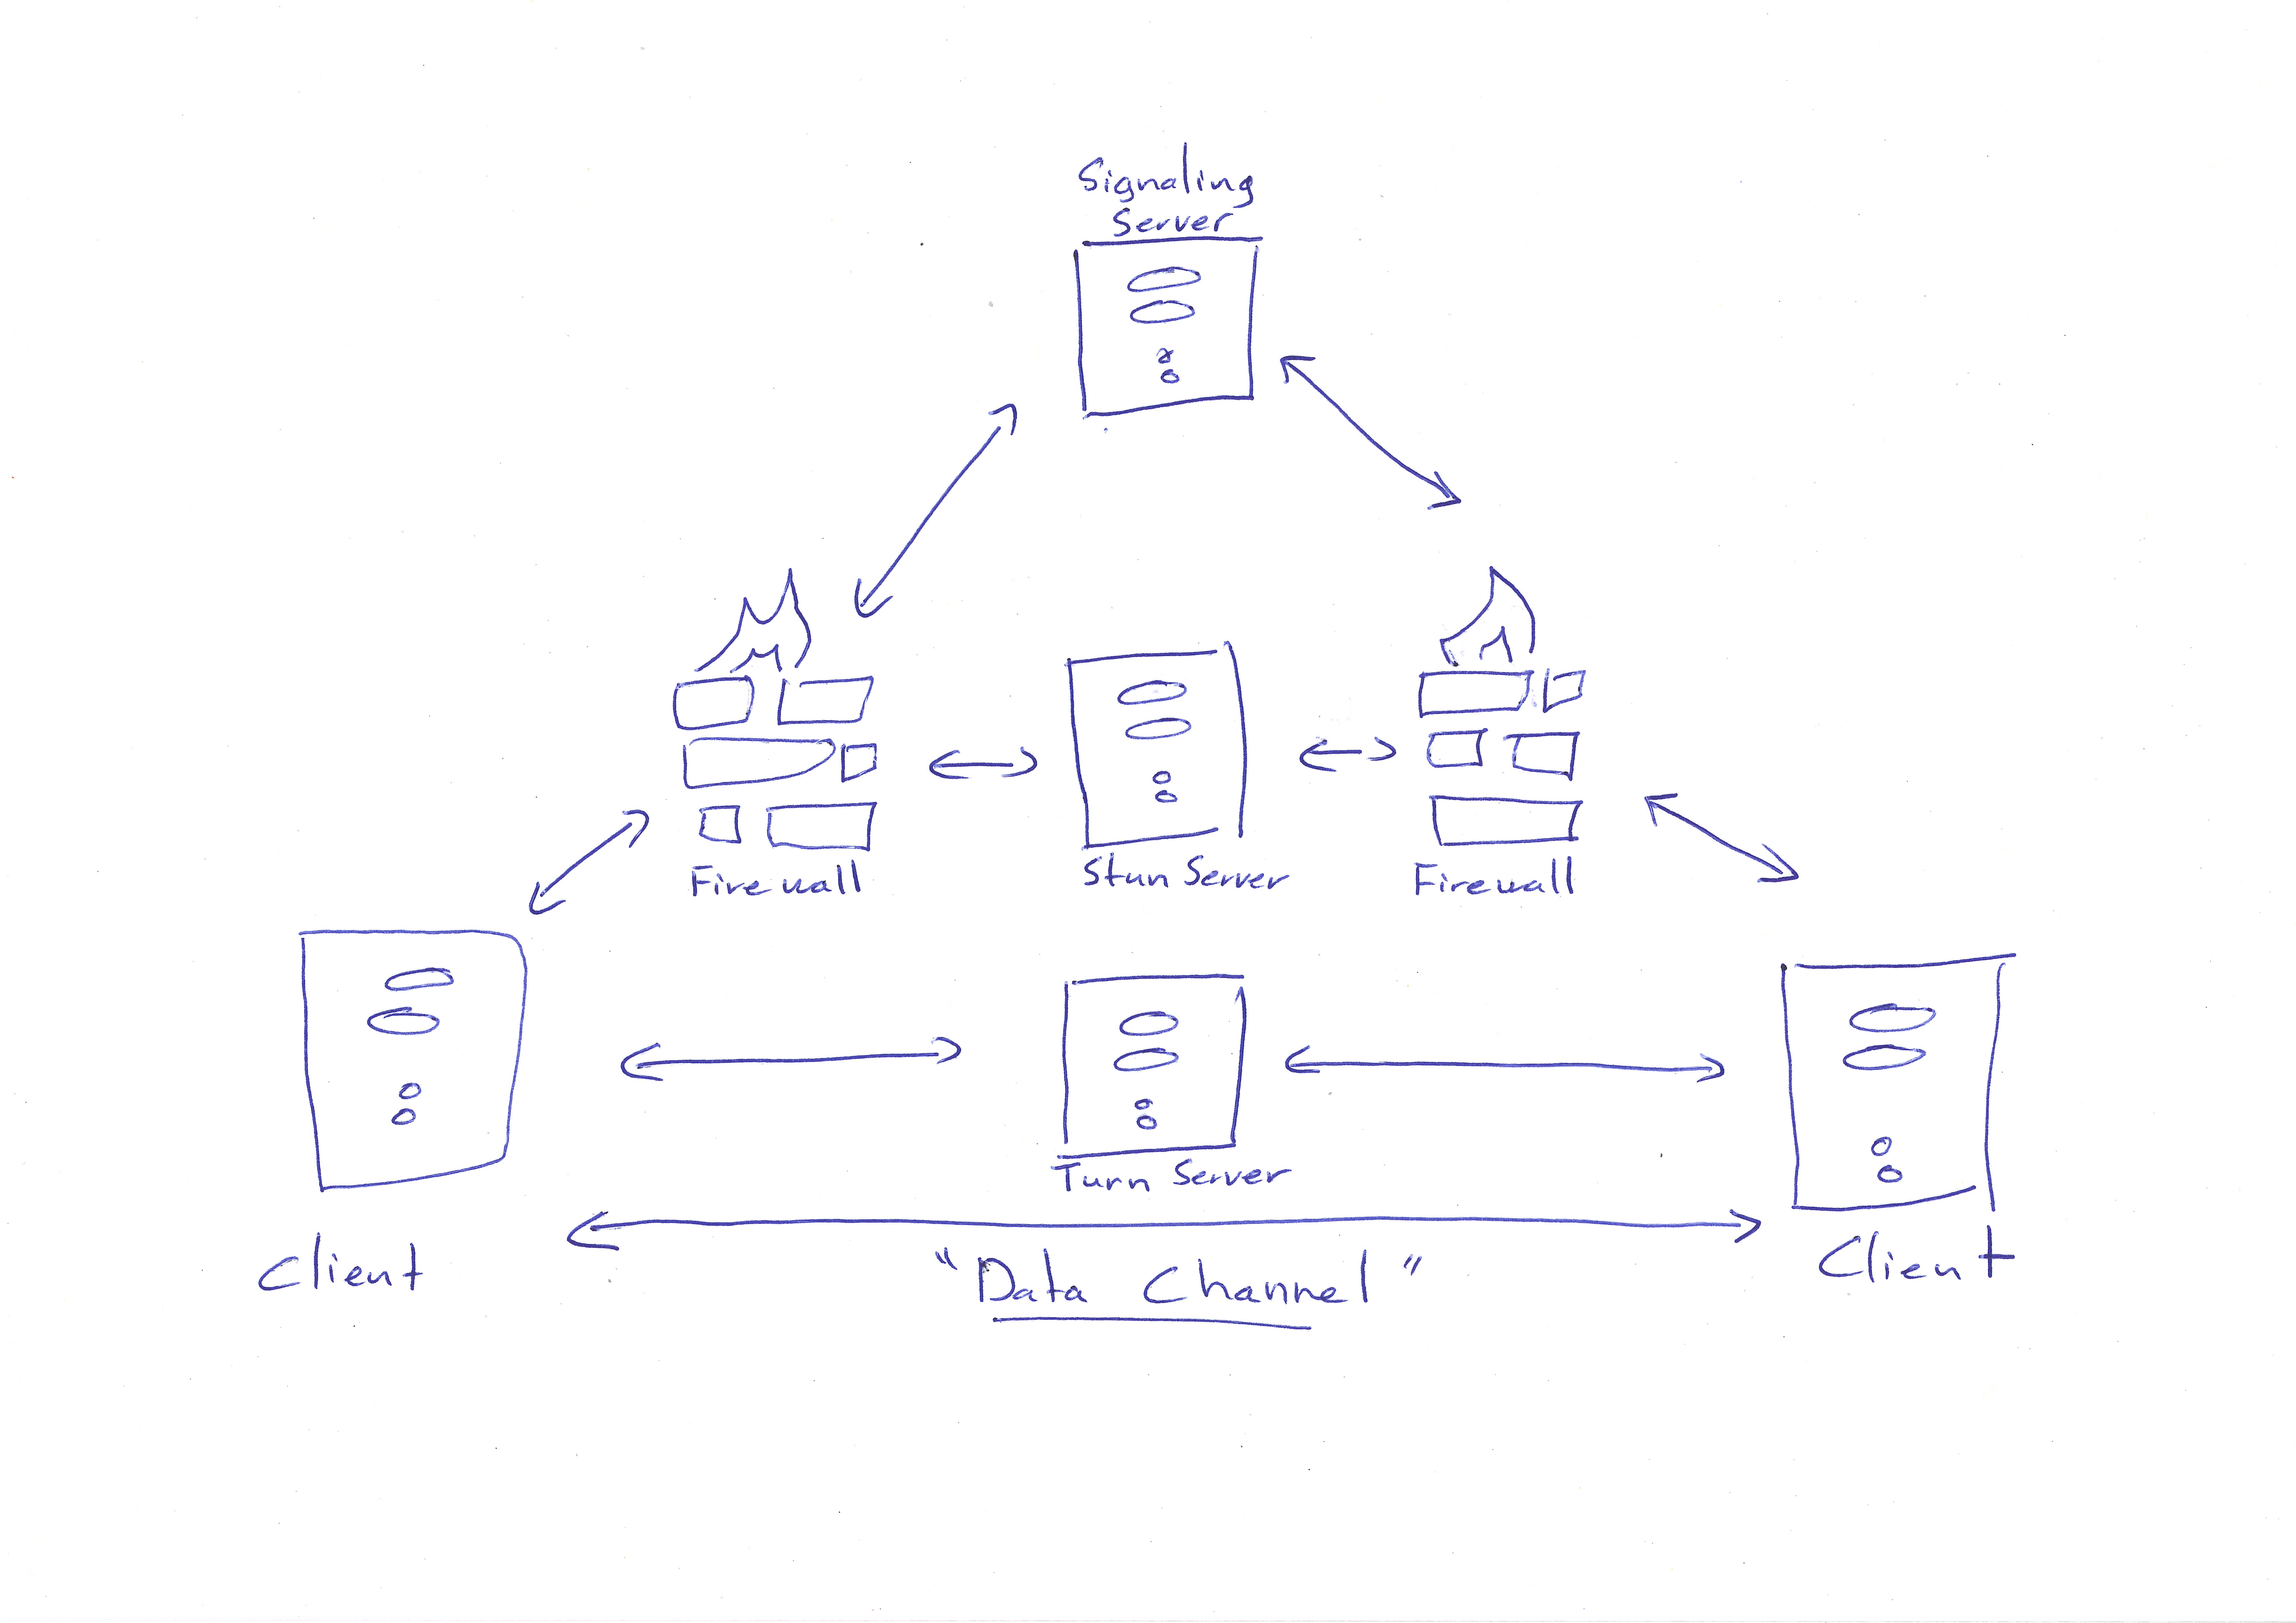
\includegraphics[scale=0.1]{annexes/schemes/signaling-basic.jpg}
\end{adjustbox}
\end{figure} 

\subsubsection{Tracker} In the goal to avoid a centralization of the signaling server, we tried looked into solutions for homemade trackers. The results theoretically solutions were to use GitHub or Twitter has a listing. However, research led us to an already existing similar technology WebTorrent\cite{Torrent2015WebTorrent}. We tested this solution, the client (browser) is connecting into a known tracker, which could be virtually run by anyone, and the client retrieves the list of connected users ids. It is the same concept as peerJS (managing the peer ids to initialize the connection between peers).

\subsubsection{Serverless} The main idea here it to use STUN servers from vast and public companies like Google to open a port that goes through the firewall to talk to the STUN server and opens a bidirectional flux. This flux is then matched with another client who did the same thing and the magic happens. Google's STUN used is \url{stun.l.google.com:19302}. 

\subsubsection{Live} It's possible to try the PeerJS version from this public URL address \url{http://rocla.github.io/OverClouds-public}
Note that we chose not to release the serverless solution to the public yet.

%-------------------------------------------------------
%    END OF COMMUNICATION
%-------------------------------------------------------